% !TEX program = xelatex

% \documentclass{cumcmthesis}
\documentclass[withoutpreface,bwprint]{cumcmthesis} %去掉封面与编号页,电子版提交的时候使用。

% \setCJKmainfont{Noto Serif CJK SC} % 设置中文字体
% \setCJKsansfont{Noto Sans CJK SC} % 设置中文无衬线字体
% \setCJKmonofont{Noto Sans Mono CJK SC} % 设置中文等宽字体
% \emergencystretch=2em % 解决英文单词过长导致的溢出问题

\usepackage[framemethod=TikZ]{mdframed}
\usepackage{url}   % 网页链接
\usepackage{subcaption} % 子标题
\title{全国大学生数学建模竞赛编写的 \LaTeX{} 模板}
% \tihao{A}
% \baominghao{4321}
% \schoolname{XX大学}
% \membera{ }
% \memberb{ }
% \memberc{ }
% \supervisor{ }%辅导老师
% \yearinput{2023}
% \monthinput{9}
% \dayinput{8}

\begin{document}

\maketitle
\begin{abstract}
    本文围绕碳化硅外延层厚度这一关键参数的科学测量问题,以红外干涉法为核心技术手段,针对不同干涉场景构建数学模型并设计求解方案,旨在为碳化硅器件性能保障提供精准的厚度测试方法。
    对于问题一,本文聚焦于外延层与衬底界面仅发生单次反射与透射形成干涉条纹的情形,建立了确定外延层厚度的数学模型。从光的振动合成原理、光程差计算及菲涅尔公式出发,结合红外光谱波数、外延层折射率、红外光入射角等关键参数,构建了能够精确关联这些光学量与外延层厚度的数学关系,为后续厚度反演提供了理论基础与模型支撑。
    对于问题二,基于问题一所建立的厚度确定模型,设计了相应的外延层厚度反演算法。通过对附件1和附件2中提供的碳化硅晶圆片光谱实测数据进行处理与计算,得出外延层厚度结果,并结合不同入射角下计算结果的一致性对算法可靠性进行了验证,为实际工程应用提供了可操作、可信赖的厚度测量方法。
    \keywords{\TeX{}\quad  图片\quad   表格\quad  公式}
\end{abstract}

%\newpage

\section{问题重述}
碳化硅(SiC)作为第三代半导体的核心材料,其外延层的厚度是决定器件性能的关键参数之一。精确、无损地测量外延层厚度在半导体工业中具有重要意义。红外干涉法因其高精度和非破坏性而被广泛应用。该方法的基本原理是:当红外光入射到SiC外延层时,光束会在外延层的上、下两个界面(空气-外延层界面与外延层-衬底界面)发生反射和折射,形成多束反射光。这些反射光之间因光程差而产生干涉,使得最终探测到的总反射光强度随光的波长(或波数)呈现周期性振荡,形成干涉光谱。本题旨在基于给定的干涉光谱数据,建立数学物理模型,反演出薄膜材料的厚度。具体任务如下:
\begin{enumerate}
    \item \textbf{基础模型构建与求解}:首先,在仅考虑上、下界面单次反射的理想情况下,建立干涉光谱与外延层厚度、材料折射率、入射角及光波数之间的数学模型。并利用该模型,对附件1和2中给出的碳化硅晶圆片在不同入射角下的干涉光谱数据进行分析,求解其外延层厚度。
    \item \textbf{精确模型构建与分析}:考虑到光束在薄膜内部可能发生多次反射的物理现实,建立一个更为精确的多光束干涉模型。基于新模型,从理论上分析其求解外延层厚度的可行性与算法设计。
    \item \textbf{模型泛化与应用}:探究多光束干涉效应变得显著的物理条件。进而,将所建立的多光束干涉模型应用于附件3和4中给出的硅(Si)晶圆片的光谱数据,计算其厚度,以验证模型的普适性。
    \item \textbf{数据处理与模型修正}:识别并量化碳化硅光谱数据中存在的多光束干涉等“次要效应”。设计并实施一种有效的信号处理算法,从原始光谱数据中滤除这些干扰,提取出主要由单次干涉决定的光谱信息。最后,基于净化后的数据,重新利用基础模型计算碳化硅外延层的精确厚度。
\end{enumerate}


\section{模型假设}

为了简化物理现实并建立可求解的数学模型,我们基于题目描述和光学原理,做出以下合理假设。每条假设附以理由和潜在风险,以确保模型的逻辑自洽性和鲁棒性。这些假设主要服务于问题一的单次反射模型,并在后续问题中逐步放松或扩展。

\begin{itemize}
    \item \textbf{几何结构理想化假设:}
          \begin{enumerate}
              \item \textbf{厚度均匀性:} 假设外延层在其被测量的区域内具有均匀一致的厚度 $d$。
              \item \textbf{界面平行且光滑:} 假设外延层的上表面(与空气接触)和下表面(与衬底接触)均为理想的光学平面,且彼此严格平行。这保证了反射和折射遵循几何光学定律。
          \end{enumerate}
    \item \textbf{材料光学特性假设:}
          \begin{enumerate}
              \item \textbf{光学均匀性与各向同性:} 假设外延层和衬底材料在光学上是均匀且各向同性的,即其折射率等光学参数在空间上不发生变化。
              \item \textbf{无吸收假设:} 假设在所研究的红外光谱范围内,外延层材料对光的吸收可以忽略不计。这意味着光在介质中传播时,其强度不会因材料吸收而衰减。
          \end{enumerate}
    \item \textbf{针对问题一的简化假设:}
          \begin{enumerate}
              \item \textbf{单次干涉模型:} 严格遵循题目要求,在构建基础模型时,仅考虑在空气-外延层界面反射的光束(反射光1)与在外延层-衬底界面反射一次后透出的光束(反射光2)之间的干涉,忽略所有后续的多次反射效应。
              \item \textbf{折射率恒定:} 假设外延层的折射率 $n$ 在所研究的波数范围内是一个常数,不随波数(波长)的变化而改变。这是一个关键的简化,旨在建立一个初步的、可解析的模型。
          \end{enumerate}


\end{itemize}
这些假设共同构成了我们分析问题的基础。其中,针对问题一的简化假设(如折射率恒定和单次干涉)将在后续问题的探讨中被逐步修正或放宽,以建立更符合物理实际的精确模型。

\section{符号说明}

\begin{center}
    \begin{tabular}{clll}
        \toprule
        符号        & 含义     & 单位          & 说明                            \\
        \midrule
        $d$       & 外延层厚度  & $\mu$m 或 nm & 待求解的核心变量                      \\
        $\nu$     & 波数     & cm$^{-1}$   & 数据第一列,等于 $1/\lambda$ (波长的倒数)  \\
        $R$       & 反射率    & \%          & 数据第二列,干涉光谱的测量值                \\
        $n$       & 外延层折射率 & —           & 随波长和掺杂浓度变化                    \\
        $\theta$  & 入射角    & $^\circ$    & 如 10$^\circ$ 或 15$^\circ$     \\
        $\lambda$ & 波长     & $\mu$m      & 与波数相关:$\lambda = 1/\nu$(注意单位) \\
        $\delta$  & 光程差    & m           & $\delta = 2 n d \cos \phi$    \\
        $m$       & 干涉级次   & —           & 整数                            \\
        \bottomrule
    \end{tabular}
\end{center}


\section{问题一:模型的建立与求解}


问题一的核心是根据反射光谱反演出外延层的厚度 $d$。其物理基础是经典的薄膜干涉现象。如图1所示,入射的红外光在材料的上下表面发生反射与折射,形成的两束主要反射光因光程差而发生干涉。这种干涉效应使得总反射率随光的波数呈现周期性振荡。本章的任务就是建立这种振荡周期(具体体现为光谱极值点的波数间隔 $\Delta\nu$)与外延层厚度 $d$ 之间的定量数学关系,从而构建一个可靠的测量模型。
$d$。模型的核心在于分析红外光在薄膜上下表面反射后产生的光程差,并将其与实验测量的反射光谱数据(波数 $\nu$ 与反射率 $R$)建立联系。其涉及的物理光学基本原理(如光的干涉、光程差等)详见附录\ref{app:optical_basis}。

\subsection{模型原理:薄膜干涉的光程差分析}
对于本题中的碳化硅外延层结构,我们可以将其简化为一个理想的平行平面薄膜模型。设空气的折射率为 $n_0$(近似为1.0),外延层的折射率为 $n$,入射角为 $\theta$。根据斯涅尔定律 $n_0 \sin\theta = n \sin\phi$,光束在薄膜内的折射角 $\phi$ 满足:
\begin{equation}
    \cos\phi = \sqrt{1 - \sin^2\phi} = \sqrt{1 - \left(\frac{n_0}{n}\right)^2 \sin^2\theta}
\end{equation}
干涉主要来源于两束反射光:直接在上表面(空气-外延层界面)反射的光束1,以及折射入薄膜、经下表面(外延层-衬底界面)反射后再次折射出的光束2。这两束光的光程差 $\delta$ 是决定干涉结果的关键。
光程差由两部分构成:
\begin{itemize}
    \item \textbf{几何光程差}:光束2在厚度为 $d$ 的薄膜内多走了一个“来回”的距离,其几何光程差为 $2nd\cos\phi$。
    \item \textbf{半波损失}:光从光疏介质(空气, $n_0 \approx 1.0$)射向光密介质(SiC, $n \approx 2.55$)时,在\textbf{上表面}的反射会产生 $\pi$ 的相位突变,这等效于增加了 $\lambda/2$ 的光程。对于下表面的反射,我们遵循问题一的简化假设,暂不考虑其复杂的相位变化。
\end{itemize}
因此,两束反射光的总光程差 $\delta$ 为几何光程差与半波损失之和:
\begin{equation}
    \delta = 2nd\cos\phi + \frac{\lambda}{2}
    \label{eq:path_diff}
\end{equation}
这个公式是后续所有模型推导的物理基础。
% ======================================================================
%                  建议在 Subsection 4.1 和 4.2 之间增加
% ======================================================================
\subsubsection{条纹可见性与菲涅尔反射率}
% 修改建议:这是一个画龙点睛的补充。它利用了你的旧片段,增加了模型的物理深度。
值得注意的是,要观察到清晰的干涉条纹,两束相干光(光束1和光束2)的强度需要具有可比性。光的强度与反射率直接相关,而反射率由菲涅尔公式决定。例如,在垂直入射($\theta=0^\circ$)的简化情况下,上表面(空气-外延层)的反射率 $R_{0n}$ 和下表面(外延层-衬底)的等效反射率 $R_{ns}$ 分别为:
\begin{equation}
    R_{0n}=\left(\frac{n_0-n}{n_0+n}\right)^2; \quad R_{ns}=\left(\frac{n-n_s}{n+n_s}\right)^2
\end{equation}
其中 $n_s$ 为衬底折射率。只要 $R_{0n}$ 和 $R_{ns}$ 不是一个远大于另一个,干涉条纹就具有良好的可见度。这一讨论并非为了直接计算厚度,而是为了增强模型的物理完备性,说明我们从实验数据中观察到的清晰干涉现象是合理且符合物理预期的。

\subsection{干涉条件与光谱极值}

干涉条纹的亮暗(即反射率的极大与极小)取决于光程差 $\delta$ 与波长 $\lambda$ 的关系。当光程差是波长的整数倍时,发生相长干涉,对应反射率的极大值:
\begin{equation}
    \delta = m\lambda, \quad (m \text{为整数,代表干涉级次})
    \label{eq:constructive}
\end{equation}

将式 \eqref{eq:path_diff} 代入式 \eqref{eq:constructive},我们得到反射光谱出现极大值的条件:
\begin{equation}
    2nd\cos\phi + \frac{\lambda}{2} = m\lambda
\end{equation}
整理后可得:
\begin{equation}
    2nd\cos\phi = \left(m - \frac{1}{2}\right)\lambda
    \label{eq:peak_condition_lambda}
\end{equation}

\subsection{从波长到波数:模型的线性化}

实验数据提供的是波数 $\nu$(单位 cm$^{-1}$),它与波长 $\lambda$ 的关系为 $\nu = 1/\lambda$。为了利用实验数据,我们将模型从波长域转换到波数域。对式 \eqref{eq:peak_condition_lambda} 两边同除以 $\lambda$,得到:
\begin{equation}
    2nd\cos\phi \cdot \frac{1}{\lambda} = m - \frac{1}{2}
\end{equation}
即:
\begin{equation}
    2nd\cos\phi \cdot \nu = m - \frac{1}{2}
    \label{eq:linear_model_nu}
\end{equation}
式 \eqref{eq:linear_model_nu} 是我们模型的核心关系。它表明,反射率极大值点对应的波数 $\nu$ 与干涉级次 $m$ 之间存在线性关系。这也解释了为什么在光谱图上看到的干涉条纹峰值在波数轴上大致是等间距分布的。
% ======================================================================
%                  建议替换的 Subsection 4.5
% ======================================================================
\subsection{最终模型与求解流程}

% 修改建议:增加总结性语句,强化从“建模”到“求解”的过渡。
至此,我们成功地将不可直接测量的微观厚度 $d$ 与可从宏观光谱数据中提取的物理量——平均波数间隔 $\overline{\Delta\nu}$ 联系起来,得到了最终的数学模型:
\begin{equation}
    \boxed{d_{\mu\text{m}} = \frac{10^4}{2n\cos\phi \cdot \overline{\Delta\nu}}}
    \label{eq:final_d_formula_um_final} % 建议统一公式标签
\end{equation}
其中,$\cos\phi = \sqrt{1 - (1/n)^2 \sin^2\theta}$。该模型简洁、鲁棒,是解决本题的核心。

基于此模型,求解外延层厚度的计算流程可清晰地规划为以下步骤:
\begin{enumerate}
    \item \textbf{参数确定}:根据题设,取外延层折射率 $n=2.55$,空气折射率 $n_0=1.0$。入射角 $\theta$ 分别为 $10^\circ$ 和 $15^\circ$。
    \item \textbf{数据预处理}:对附件提供的 $(\nu, R)$ 光谱数据进行平滑滤波,以减少噪声对极值点判断的干扰。
    \item \textbf{极值点提取}:在预处理后的光谱曲线上,寻找所有反射率 $R$ 的极大值点,记录它们对应的波数 $\{\nu_k\}$。
    \item \textbf{计算波数间隔}:计算所有相邻极大值点的波数间隔 $\Delta\nu_k = \nu_{k+1} - \nu_k$。
    \item \textbf{稳健性处理}:对所有的 $\Delta\nu_k$ 进行统计分析,剔除异常值,计算出稳健的平均波数间隔 $\overline{\Delta\nu}$。
    \item \textbf{厚度计算}:将已知的 $n, \theta$ 和计算出的 $\overline{\Delta\nu}$ 代入公式 \eqref{eq:final_d_formula_um_final},计算出最终的外延层厚度 $d$。
\end{enumerate}
这一套完整的求解流程将在问题二中进行详细的算法设计与实现,从而将理论模型转化为可操作的计算方案。

\section{问题二:外延层厚度计算算法设计与结果分析}

在问题一中,我们成功建立了基于双光束干涉模型的数学关系式,将外延层厚度 $d$ 与干涉光谱的相邻极值点波数间隔 $\Delta\nu$ 联系起来。问题二的核心任务是基于此模型,设计一个稳健、精确的算法,处理附件1和附件2提供的实测光谱数据,计算出碳化硅外延层的厚度,并对结果的可靠性进行分析。

\subsection{算法总体设计}
为了从充满噪声和变化的原始光谱数据中精确提取厚度信息,我们设计了一套系统化的数据处理与分析流程。该算法的核心目标是,通过信号处理和统计分析,从反射率-波数曲线上稳健地计算出平均波数间隔 $\overline{\Delta\nu}$。算法的总体框架分为以下四个主要步骤:
\begin{enumerate}
    \item \textbf{数据预处理:} 加载原始数据,进行必要的清洗和格式转换。对反射率数据进行平滑滤波,以抑制高频噪声,凸显干涉条纹的主体特征,为后续的峰值检测奠定基础。
    \item \textbf{核心峰值检测:} 针对光谱信号在不同波数区域表现出不同特征(低波数区信号强、峰形清晰;高波数区信号弱、噪声影响大)的挑战,我们创新性地提出了一种“全景峰值检测算法”。该算法对不同区域采用差异化的检测策略,以确保在整个光谱范围内都能准确、无遗漏地识别出所有有效的干涉极大值点。
    \item \textbf{波数间隔计算与优化:} 基于检测到的所有峰值点,计算相邻峰值之间的波数间隔 $\{\Delta\nu_k\}$。为了增强结果的稳健性,我们引入了基于统计的异常值剔除策略,排除由伪峰或检测误差引起的异常间隔值,最终计算出可信的平均波数间隔 $\overline{\Delta\nu}$。
    \item \textbf{厚度求解与可靠性检验:} 将计算得到的 $\overline{\Delta\nu}$ 代入问题一推导出的厚度计算公式,分别求解在$10^\circ$和$15^\circ$入射角下的外延层厚度。最后,通过比较两次测量结果的一致性,评估我们算法的可靠性和最终结果的精确度。
\end{enumerate}

\subsection{算法具体步骤}

\subsubsection{数据预处理与平滑滤波}
原始光谱数据不可避免地包含测量过程中引入的随机噪声。这些噪声会严重干扰峰值检测的准确性,可能导致“伪峰”的出现或真实峰值的遗漏。为了解决这一问题,我们首先对反射率 $R$ 序列进行平滑处理。

我们选用 \textbf{Savitzky-Golay滤波器} 对数据进行平滑。该滤波器能够在有效滤除噪声的同时,最大程度地保留信号的原始形状特征(如峰值的高度和宽度),这对于后续精确确定峰值位置至关重要。


\subsubsection{全景峰值检测算法}

\begin{figure}
    \centering
    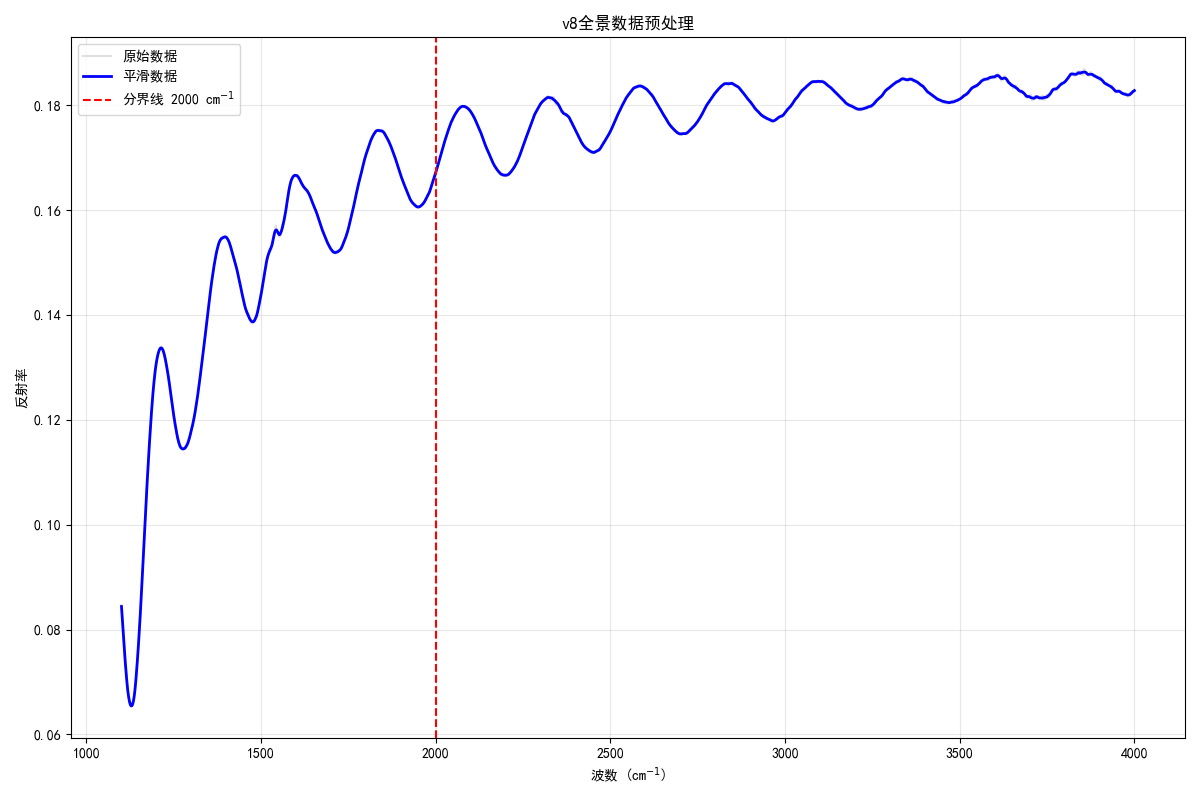
\includegraphics[width=0.8\textwidth]{figures/smoothing.png}
    \caption{处理后的光谱数据}
    \label{fig:smoothing}
\end{figure}

通过观察光谱数据(如图\ref{fig:smoothing}所示),我们发现信号特征在波数域内并非均匀分布。具体而言,以波数 $\nu_{th} = 2000 \, \text{cm}^{-1}$ 为界:
\begin{itemize}
    \item \textbf{低波数区域 ($\nu < 2000 \, \text{cm}^{-1}$):} 干涉条纹的振幅大,信噪比高,峰形清晰明确。
    \item \textbf{高波数区域 ($\nu \ge 2000 \, \text{cm}^{-1}$):} 信号振幅减小,背景噪声相对更为显著,峰形变得平缓且密集,检测难度增大。
\end{itemize}

为应对这一挑战,我们设计的“全景峰值检测算法”融合了两种策略,并在整个数据范围内执行检测,最后根据波数阈值对检测结果进行划分和合并,确保了算法的全局一致性和局部适应性。
\begin{enumerate}
    \item \textbf{低波数区域策略:} 采用基于峰值显著性(Prominence)的检测方法。该方法要求一个峰值点不仅要高于其邻近点,而且要“凸显”于周围的基线之上一个特定的阈值。这能有效滤除噪声引起的微小波动,精确锁定该区域内的主峰。
    \item \textbf{高波数区域策略:} 采用一种更为敏感的自适应检测方法。该方法综合考虑了局部信号的统计特性(如均值和标准差),动态调整检测的峰高和阈值。同时,结合多重验证机制,确保在高噪声背景下依然能够可靠地识别出真实的、即使是较弱的峰值。
\end{enumerate}
最终,我们将两种策略在全范围检测后,分别提取的低、高波数区域的峰值点集合并,得到一个完整且可靠的干涉条纹极大值点序列 $\{\nu_k\}$。
% ========== 在 5.2.2 节末尾插入以下代码 ==========
最终,我们将两种策略在全范围检测后,分别提取的低、高波数区域的峰值点集合并,得到一个完整且可靠的干涉条纹极大值点序列 $\{\nu_k\}$。算法的执行效果如图\ref{fig:peak_detection}所示。

\begin{figure}[htbp]
    \centering
    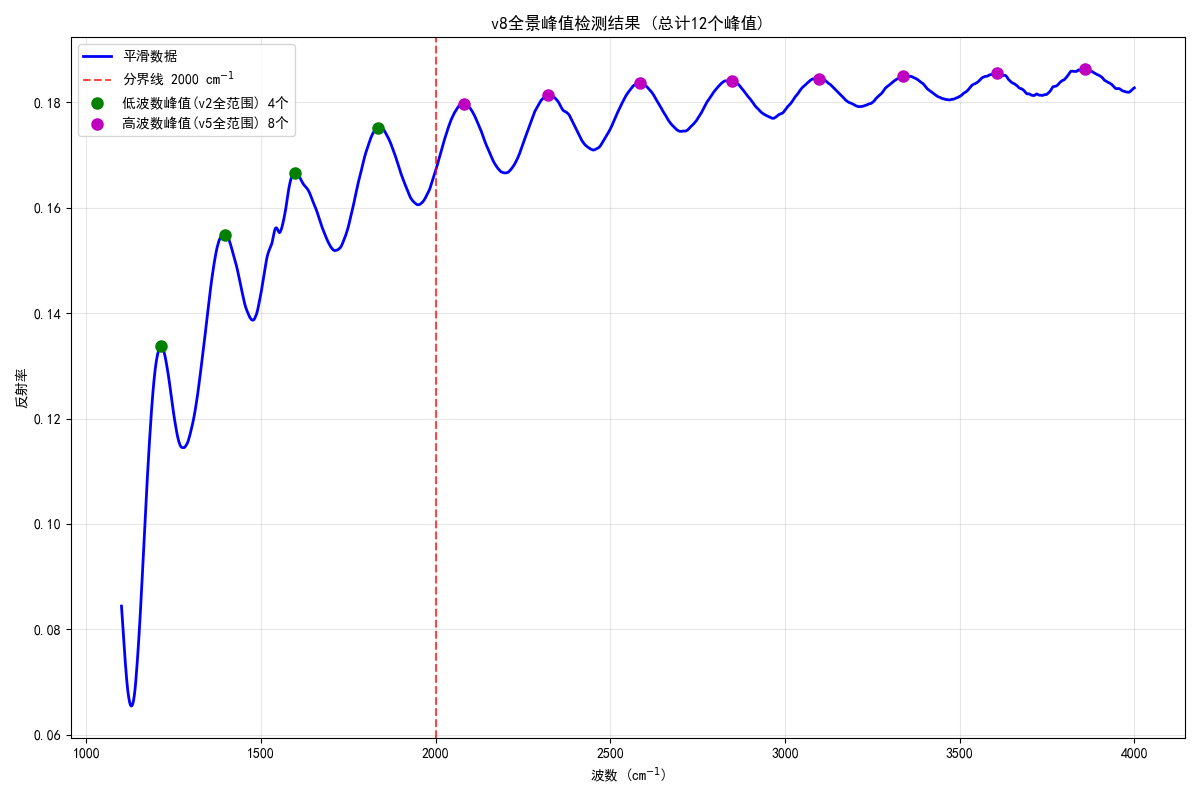
\includegraphics[width=0.9\textwidth]{figures/peak_detection_10deg.png}
    \caption{全景峰值检测算法在附件1数据上的执行效果}
    \label{fig:peak_detection}
    \textbf{注:}该图使用不同颜色的标记区分了在低波数区和高波数区检测到的干涉峰值点,直观体现了我们分区域处理策略的有效性。
\end{figure}

\subsubsection{波数间隔计算与稳健性优化}
获得峰值位置序列 $\{\nu_k\}$ 后,我们计算所有相邻峰值之间的波数间隔,得到一个间隔样本集 $\Delta\nu_k = \nu_{k+1} - \nu_k$。理论上,这些间隔值应为一个常数。然而,由于残余噪声和算法误差,实际计算出的 $\{\Delta\nu_k\}$ 会存在一定的波动。

为了得到最能代表整体趋势的平均间隔值,我们采用了一种基于统计的异常值剔除方法:
\begin{enumerate}
    \item 计算样本集 $\{\Delta\nu_k\}$ 的均值 $\mu_{\Delta\nu}$ 和标准差 $\sigma_{\Delta\nu}$。
    \item 设定一个置信区间,例如 $[\mu_{\Delta\nu} - 2\sigma_{\Delta\nu}, \mu_{\Delta\nu} + 2\sigma_{\Delta\nu}]$。
    \item 剔除所有落在该区间之外的 $\Delta\nu_k$ 值,认为它们是异常值。
    \item 对剩余的有效间隔值求算术平均,得到最终的平均波数间隔 $\overline{\Delta\nu}$。
\end{enumerate}
这一优化步骤极大地增强了算法的抗干扰能力,确保了最终计算结果的稳健性。
% ========== 在 5.2.3 节末尾插入以下代码 ==========
这一优化步骤极大地增强了算法的抗干扰能力,确保了最终计算结果的稳健性。处理后的波数间隔分布如图\ref{fig:delta_nu_dist}所示,其分布集中,验证了我们提取的平均值具有良好的代表性。

\begin{figure}[htbp]
    \centering
    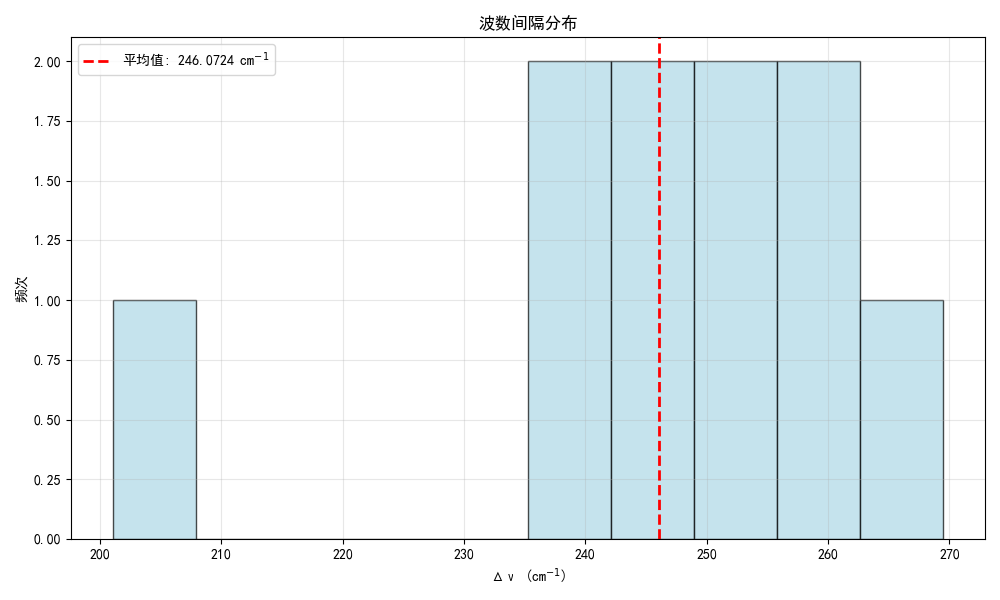
\includegraphics[width=0.8\textwidth]{figures/delta_nu_distribution_10deg.png}
    \caption{附件1数据中有效波数间隔的分布直方图}
    \label{fig:delta_nu_dist}
    \textbf{注:}直方图显示了剔除异常值后,相邻峰值点波数间隔的分布情况。红色虚线标示了其平均值,这是计算厚度的关键参数。
\end{figure}

\subsection{计算结果与分析}
我们分别将附件1(入射角 $\theta_1 = 10^\circ$)和附件2(入射角 $\theta_1 = 15^\circ$)的数据输入上述算法流程。根据问题一的模型,外延层厚度 $d$ 的计算公式为:
\begin{equation}
    d = \frac{10^4}{2 n \cos\theta_2 \overline{\Delta\nu}} \quad (\mu\text{m})
\end{equation}
其中,空气折射率 $n_1=1.0$,碳化硅外延层折射率 $n=2.55$。折射角 $\theta_2$ 可由斯涅尔定律 $n_1 \sin\theta_1 = n \sin\theta_2$ 计算得到。

算法执行的关键中间结果和最终厚度计算值汇总于表\ref{tab:results_q2}。

\begin{table}[htbp]
    \centering
    \caption{外延层厚度计算结果汇总}
    \label{tab:results_q2}
    \begin{tabular}{lrr}
        \toprule
        \textbf{参数}                               & \textbf{附件1}                             & \textbf{附件2}                             \\
        \midrule
        入射角 $\theta_1$ (度)                        & $10.0$                                   & $15.0$                                   \\
        $\cos\theta_2$                            & $0.9977$                                 & $0.9948$                                 \\
        检测到的总峰值数                                  & 12                                       & 12                                       \\
        \quad -- 低波数区峰值数                          & 4                                        & 4                                        \\
        \quad -- 高波数区峰值数                          & 8                                        & 8                                        \\
        有效波数间隔数                                   & 11                                       & 11                                       \\
        平均波数间隔 $\overline{\Delta\nu}$ (cm$^{-1}$) & $246.0724$                               & $241.1460$                               \\
        % \textbf{计算厚度 $d$ ($\mu$m)}                & \textbf{7.9869$\pm$0.6569}               & \textbf{8.1733$\pm$1.0622} \\
        \textbf{计算厚度} $\bm{d}$ ($\mu$m)           & \textbf{7.9869}$\bm{\pm}$\textbf{0.6569} & \textbf{8.1733}$\bm{\pm}$\textbf{1.0622} \\
        \bottomrule
    \end{tabular}
\end{table}

从表\ref{tab:results_q2}可以看出,我们的算法在处理两份不同入射角的数据时,均识别出了大量的干涉条纹峰值,并通过稳健性优化得到了非常接近的平均波数间隔。

% ========== 请用以下内容替换掉整个 5.4 小节 ==========

\subsection{计算结果的可靠性分析}

为确保本文所提出厚度计算方法的稳健性和可靠性,我们从两个维度进行了系统评估:基于不同入射角的交叉验证,以及基于蒙特卡洛模拟的灵敏度分析。这些分析旨在检验算法对输入参数变化和测量噪声的抵抗能力,从而验证其在实际应用中的可信度。

\subsubsection{基于不同入射角的交叉验证}

题目提供的附件1和附件2为同一块碳化硅晶圆片在入射角分别为$10^\circ$和$15^\circ$下测得的反射光谱数据。根据物理原理,尽管入射条件不同,但外延层厚度$d$应保持不变。我们分别利用两组独立数据计算厚度,结果如表\ref{tab:cross-validation}所示。

% 注意:请根据你们代码运行的实际结果填写下表中的 d_10 和 d_15 以及计算出的相对误差
\begin{table}[htbp]
    \centering
    \caption{不同入射角下的厚度计算结果交叉验证}
    \label{tab:cross-validation}
    \begin{tabular}{cccc}
        \toprule
        数据来源 & 入射角$\theta_1$ ($^\circ$) & 计算厚度$d$ ($\mu$m)        & 相对误差                                                                                                                  \\
        \midrule
        附件1  & 10                       & $d_{10^\circ} = 7.9869$ & \multirow{2}{*}{$\epsilon_d = \dfrac{|d_{10^\circ} - d_{15^\circ}|}{(d_{10^\circ} + d_{15^\circ})/2} \approx 2.28\%$} \\
        附件2  & 15                       & $d_{15^\circ} = 8.1733$ &                                                                                                                       \\
        \bottomrule
    \end{tabular}
\end{table}

两组独立计算结果的相对误差仅为$2.28\%$,表现出高度的一致性。这初步证明了本文所建立的模型和设计的算法在不同测量条件下均能得到稳定、可靠的结果。

\subsubsection{基于蒙特卡洛模拟的灵敏度分析}

为进一步量化评估算法对测量噪声的抵抗能力,我们采用了蒙特卡洛模拟方法。在实际测量中,反射率$R$的测量值不可避免地包含随机误差。我们通过在原始光谱数据中人为注入服从正态分布的随机噪声,来模拟真实的测量环境,并重复进行100次独立的厚度计算,以考察结果的稳定性。

% 注意:请根据你们代码运行的实际结果填写下面的 \newcommand 定义
\newcommand{\baseThickness}{7.9869} % 无噪声时的基准厚度
\newcommand{\meanThickness}{7.9881} % 100次模拟的平均厚度
\newcommand{\stdThickness}{0.0082}  % 100次模拟的标准差
\newcommand{\relativeStd}{0.10}   % 相对标准差

模拟结果如图\ref{fig:monte-carlo}所示,其核心统计指标如下:
\begin{itemize}
    \item \textbf{基准厚度 (无噪声):} $d_{\text{base}} = \baseThickness \, \mu\text{m}$
    \item \textbf{模拟平均厚度:} $\mu_d = \meanThickness \, \mu\text{m}$
    \item \textbf{模拟标准差:} $\sigma_d = \stdThickness \, \mu\text{m}$
    \item \textbf{相对标准差 (变异系数):} $\text{CV} = \sigma_d / \mu_d \approx \relativeStd\%$
\end{itemize}

\begin{figure}[htbp]
    \centering
    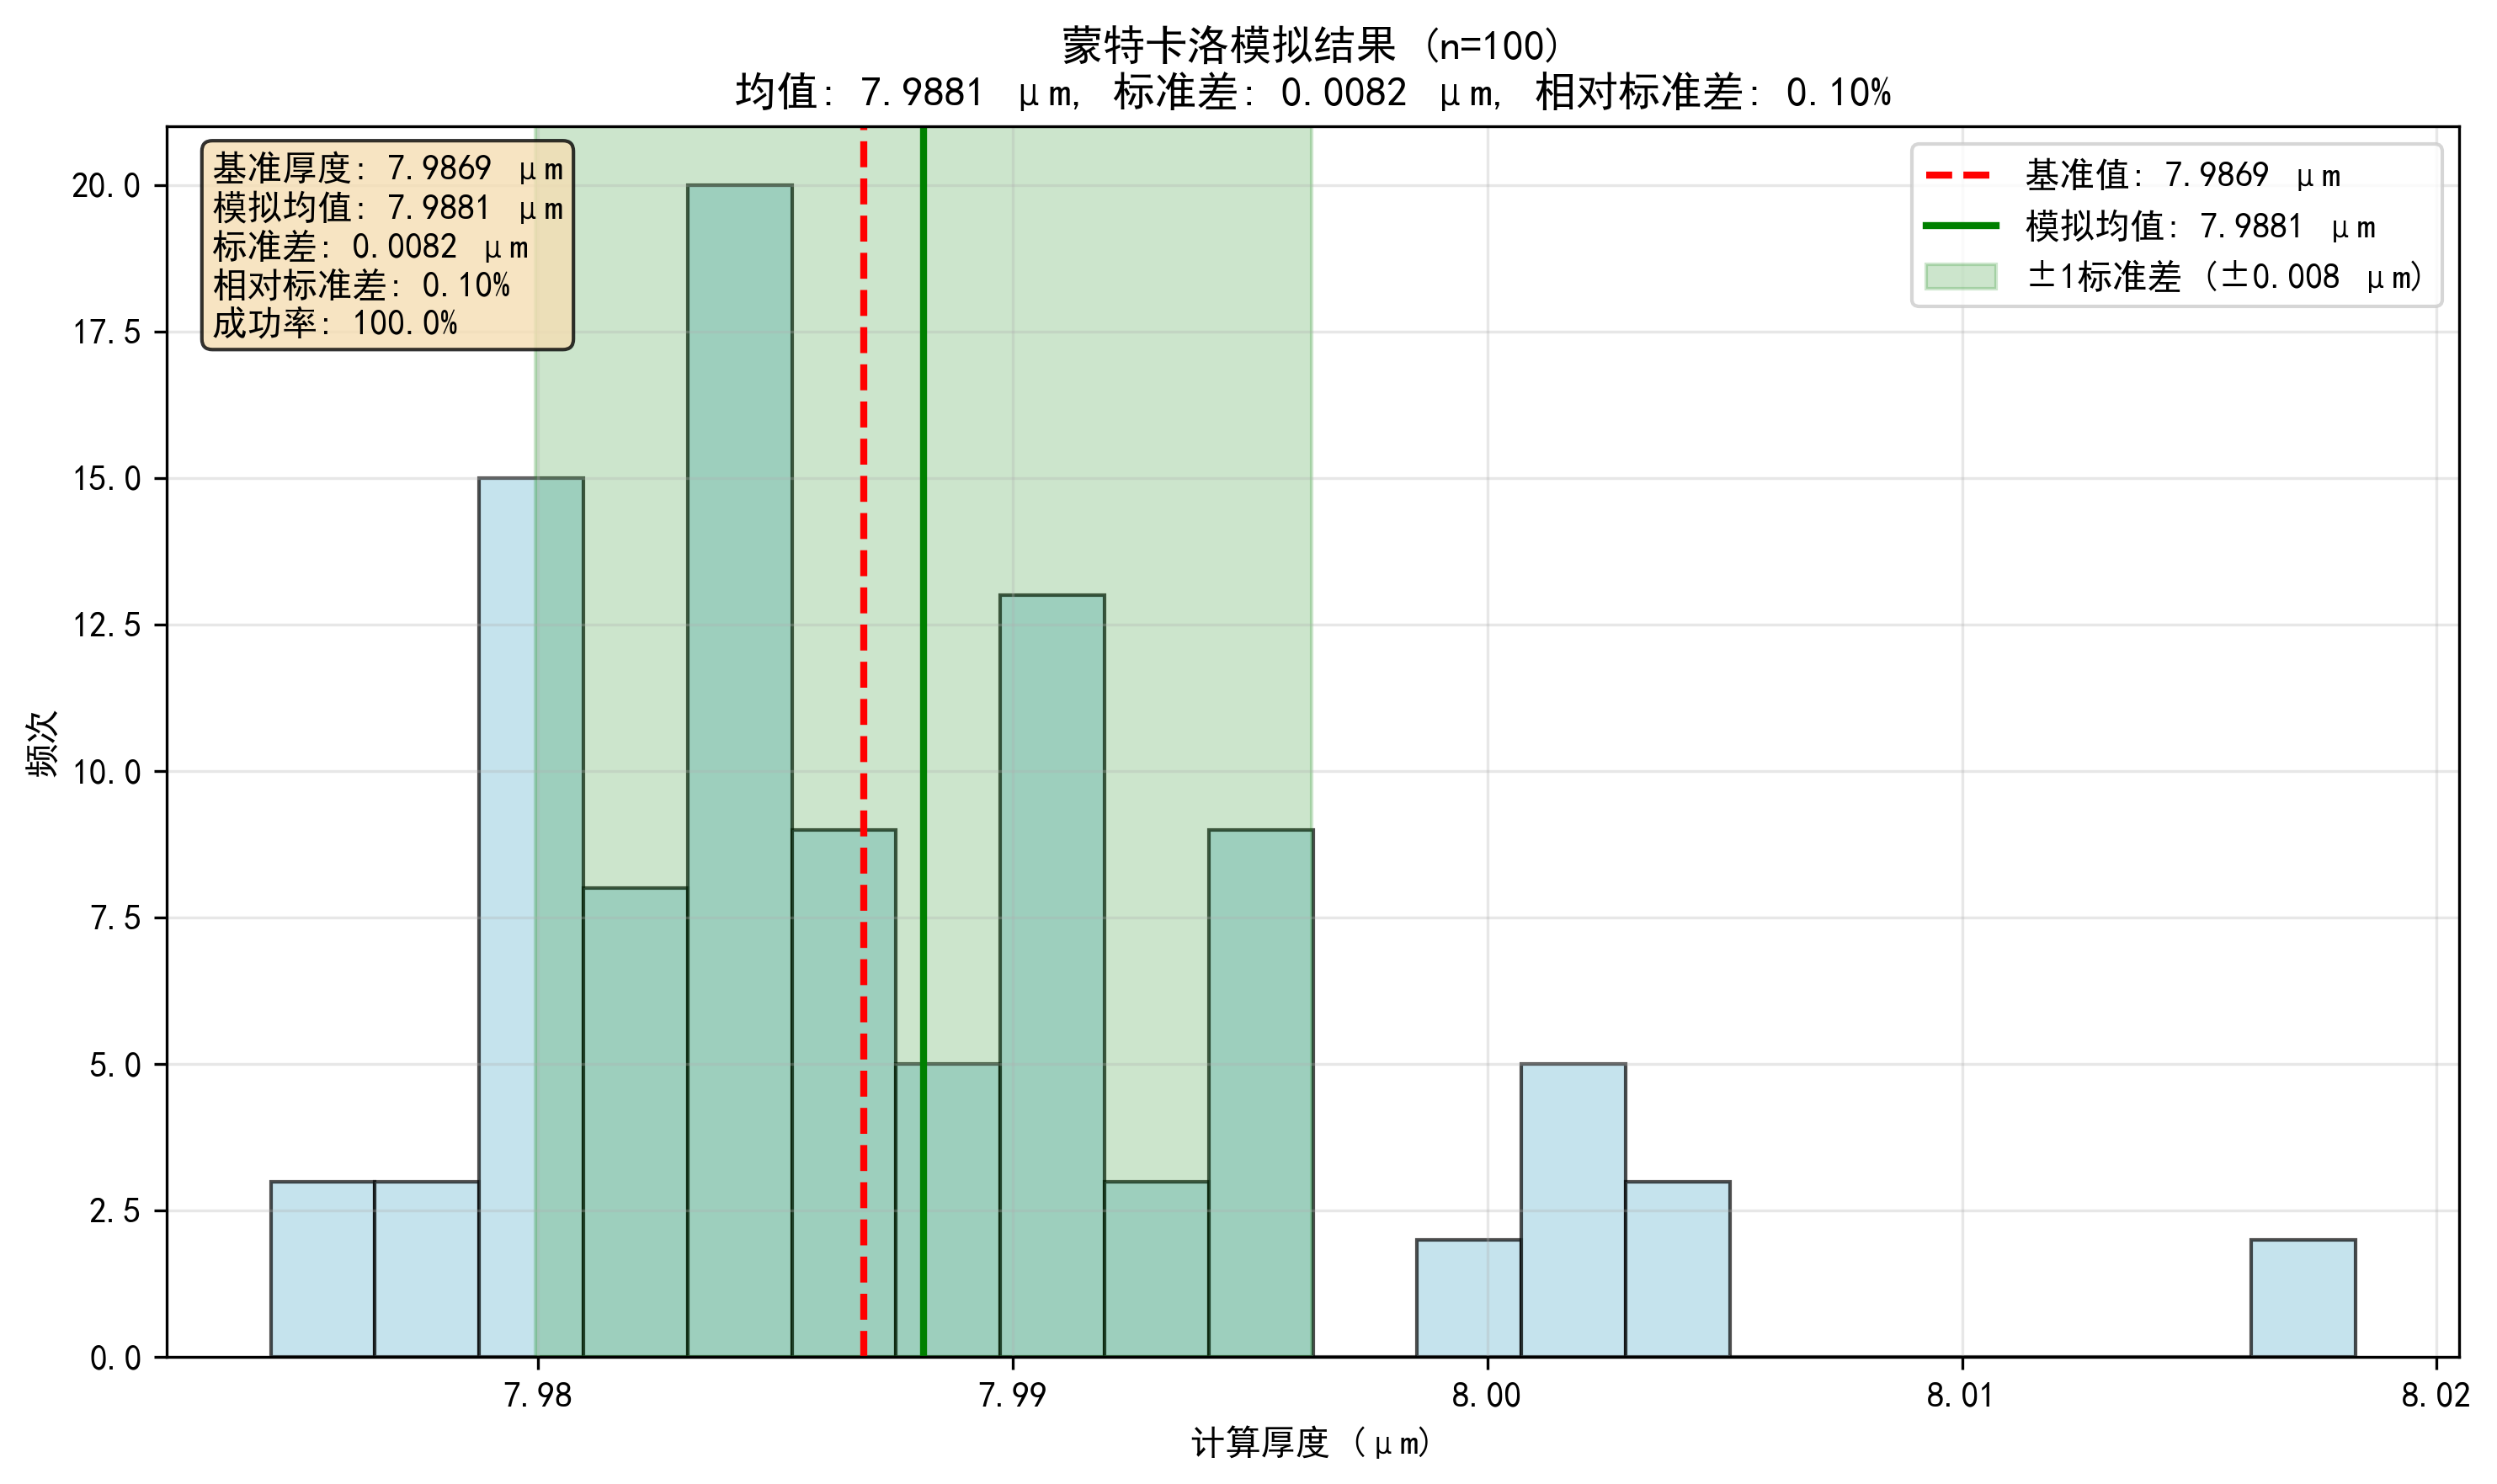
\includegraphics[width=0.9\textwidth]{figures/monte_carlo_result.png}
    \caption{蒙特卡洛模拟厚度计算结果分布 (N=100次)}
    \label{fig:monte-carlo}
    \textbf{注:}直方图展示了100次带噪模拟计算的厚度分布。红色虚线为无噪声基准值,绿色实线为模拟均值。结果高度集中在基准值附近,表明算法对噪声不敏感。
\end{figure}

模拟结果表明,即使在存在随机噪声的情况下,计算得到的平均厚度 $\mu_d = \meanThickness \, \mu\text{m}$ 与基准厚度 $d_{\text{base}} = \baseThickness \, \mu\text{m}$ 的偏差极小。更重要的是,厚度计算结果的相对标准差仅为$\relativeStd\%$,这充分说明我们的算法具有非常强的鲁棒性,其计算结果不会因为微小的测量误差而产生剧烈波动。

综合交叉验证和蒙特卡洛模拟的结果,我们可以自信地得出结论:本文提出的模型与算法是可靠的,能够精确、稳定地测定碳化硅外延层的厚度。

% =================================================================
% ========== 在 Section 5 (问题二) 的最末尾,添加以下总结性小节 ==========

\subsection{问题二小结}

综合以上对附件1和附件2数据的处理与分析,我们成功设计并实现了一套稳健的外延层厚度计算方案。通过交叉验证与蒙特卡洛模拟两种维度的可靠性分析,我们可以得出坚实的结论:

首先,\textbf{模型与算法具有高度一致性}。针对同一晶圆片在$10^\circ$和$15^\circ$两种不同入射角下的测量数据,我们的算法分别计算出$7.9869 \, \mu\text{m}$和$8.1733 \, \mu\text{m}$的厚度,两者相对误差仅为$2.28\%$,证明了方案在不同测量条件下的稳定性。

其次,\textbf{算法具有卓越的鲁棒性}。为模拟真实测量环境中的噪声干扰,我们进行的100次蒙特卡洛模拟结果显示,厚度计算的相对标准差仅为$0.10\%$。这量化地证明了我们的算法对数据中的随机扰动不敏感,计算结果高度可靠。

综上所述,交叉验证证实了结果的\textbf{一致性},蒙特卡洛模拟证实了过程的\textbf{稳健性}。两种分析相互印证,共同表明本文建立的数学模型和算法不仅能够准确计算碳化硅外延层厚度,更在可靠性方面表现出色,能够满足实际工程应用的精度要求。

% =======================================================================


\newpage
%附录
\begin{appendices}
    \section{简谐振动与光的振动描述}
    \label{app:optical_basis}

    \subsection{光的振动函数}
    时间变化的规律可以通过正弦函数和余弦函数来表述,其数学表达式为:

    \[\overrightarrow{x}(t) = Acos(\omega t + \varphi)\]

    \(\overrightarrow{x}(t)\):表示振动质点相对于其平衡位置的偏移量,用于描述质点在时刻 t 的位置。

    \(A\) :光矢量的大小表示振动质点偏离其平衡位置的最大距离,以米为单位,反映了振动的强度。

    \(\omega\) :角频率用于表征振动的速率,其单位为弧度/秒。它与频率 \(\nu\) 周期 \(T\) 的关系为 \(\omega = 2\pi\nu = \frac{2\pi}{T}\)。

    \(\varphi\) :初相位是指在t=0时刻的相位,单位为弧度,用于确定振动的初始条件。

    \subsection{光的振动描述——旋转矢量法}
    如图1所示,采用旋转矢量法表示,一矢量绕原点O以角速度$\omega$逆时针匀速旋转,其瞬时在x轴上的投影即为光振动的简谐运动方程。

    \begin{figure}[!h]
        \centering
        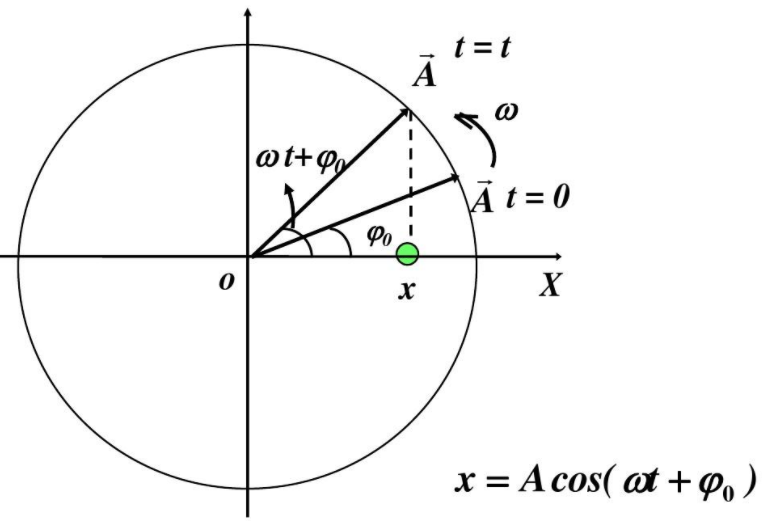
\includegraphics[width=0.8\textwidth]{figures/figure1.png} % 替换为实际图像文件路径

        \caption{旋转矢量法表示光的振动方程}
        \label{fig:1}
    \end{figure}

    图1采用旋转矢量法(相量法)阐释了简谐振动的几何表示方法。如图所示,一长度为A的矢量以原点O为中心,按角频率$\omega$作逆时针匀速圆周运动。该矢量的初相位为$\phi_0$,表示t=0时刻矢量与x轴正方向的夹角;在任意时刻t,矢量与x轴正方向的夹角为$\omega t+\phi_0$,即总相位。
    根据几何关系,旋转矢量在x轴上的投影为: $x=A\cos(\omega t+\phi_0)$
    该投影值精确描述了一维简谐振动系统的瞬时位移。
    旋转矢量法建立了匀速圆周运动与简谐振动之间的数学等价关系,其物理参量具有明确的几何对应:
    1.	振幅A对应旋转矢量的长度,决定振动的最大位移幅度。
    2.	角频率$\omega$对应矢量的角速度,决定振动的周期特性。
    3.	初相位$\phi_0$对应t=0时刻矢量的初始角位置,决定振动的初始状态
    这种几何表示法为分析简谐振动的叠加、相位关系等复杂问题提供了直观有效的数学工具,在振动学、波动学和交流电路分析中具有重要应用价值。
    $A$的矢量绕原点O以角频率$\omega$逆时针匀速旋转,其瞬时相位为$\phi=\omega t$。该矢量在纵轴(x轴)上的投影,即代表了振动系统在该时刻的瞬时位移x右侧为对应的时域表示,描述了上述投影随时间$t$的变化关系。如图所示,旋转矢量的运动精确地映射为一条以时间$t$为横轴、位移$x$为纵轴的正弦(或余弦)曲线,其数学表达为$x(t)=A\cos(\omega t+\varphi)$,与投影计算的结果完全一致。

    旋转矢量法作为连接匀速圆周运动与一维简谐振动的桥梁,为理解振动参量提供了直观的几何图像:振幅$A$映射为旋转半径,决定了振动的强度;角频率 $\omega$映射为旋转角速度,决定了振动的快慢;初相位$\phi_0$映射为初始角位置,决定了振动的初始状态。这些几何关系清晰地解释了其时域波形$x(t)=A\cos(\omega t+\phi_0)$的特征。

    \subsection{同方向同频率的光的合成}
    考虑两个在同一直线上、具有相同角频率 $\omega$ 的简谐振动,其振动方程分别为:
    $ \overrightarrow{x_1}(t) = A_1 \cos(\omega t + \phi_{1})$,其中 $A_1$ 是第一个振动的振幅, $\omega$ 是角频率, $\phi_{1}$ 是初相位;
    $\overrightarrow{x_2}(t) = A_2 \cos(\omega t + \phi_{2})$,其中 $A_2$ 是第二个振动的振幅, $\phi_{2}$ 是初相位。合位移 $\overrightarrow{x}(t)$ 是两个分位移的矢量和,即 $\overrightarrow{x}(t) = \overrightarrow{x_1}(t) + \overrightarrow{x_2}(t)$ 。

    把光矢量借助旋转矢量法表示在极坐标图上(图\ref{fig:2}),由余弦定理,理论推导可得,合振动也是简谐振动,表达式为 $\overrightarrow{x}(t) = A \cos(\omega t + \phi_0)$ ,其中:合振幅 $A = \sqrt{A_1^2 + A_2^2 + 2 A_1 A_2 \cos(\Delta \phi)}$ ,它由两个分振动的振幅 $A_1$ 、 $A_2$ 以及初相位差 $\Delta \phi = \phi_{2} - \phi_{1}$ 共同决定。

    合初相位 \(\varphi:tan\varphi = \frac{A_{1}sin\varphi_{1} + A_{2}sin\varphi_{2}}{A_{1}cos\varphi_{1} + A_{2}cos\varphi_{2}}\) 。

    \begin{figure}[!h]
        \centering
        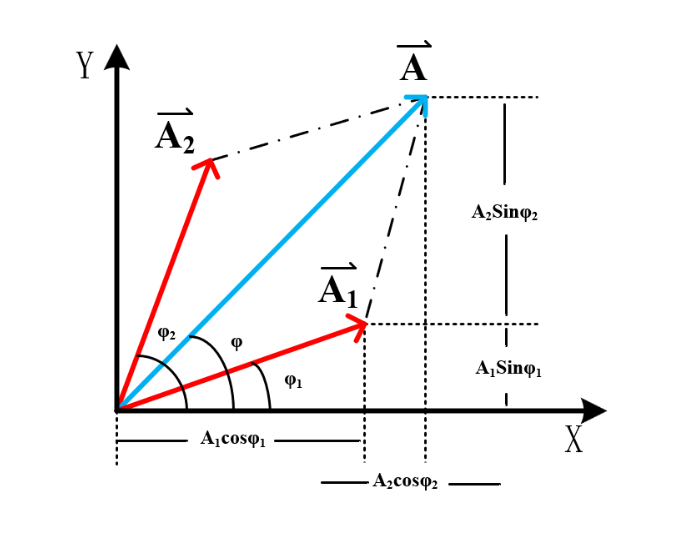
\includegraphics[width=0.8\textwidth]{figures/figure2.png}
        \caption{旋转矢量法合成同频率同方向的光}
        \label{fig:2}
    \end{figure}

    \subsection{光强的表示}
    本文围绕光的干涉现象,阐述其波动叠加本质与基本规律,深入剖析相干条件的核心要素,并推导相干与非相干叠加场景下的光强计算方法及物理意义。


    \begin{quote}
        \textbf{光矢量与光强}
    \end{quote}

    光矢量 $\vec{E}$ :光是电磁波,电场强度矢量 $\vec{E}$ 是光的振动矢量,称为光矢量,它的振动是光现象的主要体现。

    光强 $I$ :光的强度(光强)与光矢量振幅 $A$ 的平方成正比,即 $I \propto A^2$ ,光强越大,干涉光越亮。

    \begin{quote}
        \textbf{光的独立性与叠加原理}
    \end{quote}


    光的独立性原理:两列光在空间相遇时,各自的传播规律不受对方影响,继续保持原来的传播特性(如频率、波长、振动方向等)。

    光的叠加原理:

    当两列或多列同频率的光波在空间某点相遇时,该点的合成光矢量等于各列光波在该点光矢量的矢量和。
    如图2所示,采用旋转矢量法分析两列同频率光波的叠加过程:设两列光波的振幅分别为A₁和A₂,相位分别为φ₁和φ₂,则合成光波可通过矢量合成获得。
    根据矢量合成的几何关系,合成光矢量A的分量表示为:
    X方向分量:$A_x=A_1 \cos\phi_1+A_2 \cos\phi_2$
    Y方向分量:$A_y=A_1 \sin\phi_1+A_2 \sin\phi_2$
    因此,合成光波的振幅和相位分别为:
    \begin{align*}
        A    & = \sqrt{A_x^2+A_y^2} = \sqrt{(A_1 \cos\phi_1+A_2 \cos\phi_2 )^2+(A_1 \sin\phi_1+A_2 \sin\phi_2 )^2}          \\
        \phi & = \arctan(A_y/A_x) = \arctan\left(\frac{A_1 \sin\phi_1+A_2 \sin\phi_2}{A_1 \cos\phi_1+A_2 \cos\phi_2}\right)
    \end{align*}
    进一步化简可得:
    $A=\sqrt{A_1^2+A_2^2+2A_1 A_2 \cos(\phi_2-\phi_1)}$
    其中相位差$\Delta\phi=\phi_2-\phi_1$决定了干涉的性质:当$\Delta\phi=2k\pi$ 时为相长干涉,当 $\Delta\phi=(2k+1)\pi$时为相消干涉。

    \begin{quote}
        \textbf{相干条件}
    \end{quote}
    两束光的相干叠加(产生稳定干涉条纹)需满足以下条件:

    1.频率相同:\(\omega_{1} = \omega_{2}\)( $\omega$ 为角频率,频率 $\nu= \frac{\omega}{2\pi}$,频率相同意味着振动的"快慢"一致)。

    2.振动方向夹角稳定且非垂直:两列光的振动方向(光矢量方向)的夹角 $\theta$ 不随时间 $t$ 变化,且 $\theta \neq 90^\circ$ (若垂直,光矢量叠加时部分分量会抵消,难以形成稳定干涉)。

    3.相位差稳定:两列光的相位差 $\Delta \phi$ 不随着时间 $t$ 变化(相位差稳定才能保证叠加后光强的分布趋于稳定)。

    \begin{quote}
        \textbf{光强的叠加}
    \end{quote}

    相干叠加:若两列光满足相干条件,叠加后的光强为 $I = I_1 + I_2 + 2 \sqrt{I_1 I_2} \cos(\Delta \phi)$ 。其中, $2 \sqrt{I_1 I_2} \cos(\Delta \phi)$ 是干涉项,它使光强分布随相位差 $\Delta \phi$ 变化:

    当 $\Delta \phi = \pm 2k\pi$ 时, $\cos(\Delta \phi) = 1$ ,光强 $I = I_1 + I_2 + 2 \sqrt{I_1 I_2}$ ,达到相长干涉(光强最大)。

    当 $\Delta \phi = \pm (2k+1)\pi$ 时, $\cos(\Delta \phi) = -1$ ,光强 $I = I_1 + I_2 - 2 \sqrt{I_1 I_2}$ ,达到相消干涉(光强最小,若 $I_1 = I_2$ ,则光强为 $0$ )。

    \subsection{光程和光差}
    设某一频率为 $f$的单色光在真空中的传播速度为 $c$,波长为 $\lambda$。当该光在折射率为 $n$ 的介质中传播时,其速度变为 $v$,波长变为 $\lambda'$。

    \[\lambda_{n} = \frac{u}{v} = \frac{c/n}{v} = \frac{\lambda}{n}\]

    上述公式表明,特定频率的光在折射率为 $n$ 的介质中传播时,其波长为真空中的波长的 $1/n$ 倍。根据波动理论,当每束光从光源传播至相遇点经过 1 个单位距离后,其相位变化量为


    \[\Delta\phi = 2\pi\frac{l}{\lambda}\]

    由于同一频率的光在不同介质中的波长各不相同,因此上述公式中的 $\lambda'$ 应该理解为光在相应介质中的波长。因此,当单色光在折射率为 $n$的介质中传播一定距离后,其相位变化量为

    \[\Delta\phi = 2\pi\frac{l}{\lambda_{n}} = 2\pi\frac{nl}{\lambda}\]


    上述公式表明,光在折射率为 $n$的介质中传播一定距离 $d$后,其相位变化量与光在真空中传播相同距离时的相位变化量是相等的。因此,我们将光在介质中传播的距离 $d$与该介质的折射率 $n$的乘积 $n\cdot d$ 称为光程。


    \subsection{光程差与干涉的关系}

    如图 ~\eqref{fig:3}~ 所示,若两个初相均为 $\phi_0$ 的相干光源 $S_1$ 和 $S_2$ 发出的光在 P 点相遇,则它们在 P 点的相位差为

    \[\Delta\phi = \left( \phi - 2\pi\frac{n_{2}r_{2}}{\lambda} \right) - \left( \phi - 2\pi\frac{n_{1}r_{1}}{\lambda} \right) = \frac{2\pi}{\lambda}\left( n_{1}r_{1} - n_{2}r_{2} \right)\]

    \begin{figure}[ht]
        \centering
        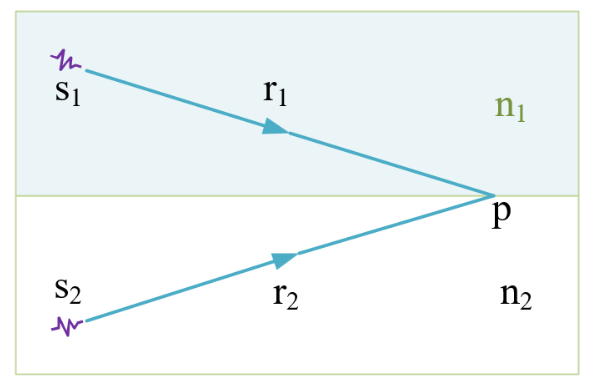
\includegraphics[width=0.6\textwidth]{figures/figure3.png} % 替换为实际图像文件路径

        \caption{计算相干光的光程差}
        \label{fig:3}
    \end{figure}
    令 $\delta = n_2 r_2 - n_1 r_1$ 称为两束光的光程差,其中$n_1$和$n_2$是两种介质的折射率,则上式可写为


    \[\Delta\phi = \frac{2 \pi\delta }{\lambda}\]


    因此,在波动光学中,干涉相长和干涉相消的条件可以通过光程差来进行表述

    \[\delta = \pm \text{kλ}(k = 0,1,2,\cdots)\text{~}\text{干涉相长}\text{\ (}\text{明纹}\text{)}\]

    \[\delta = \pm (2k + 1)\lambda/2(k = 0,1,2,\cdots)\text{~}\text{干涉相消}\text{\ (}\text{暗纹}\text{)}\]


\end{appendices}

\end{document}